\documentclass[xcolor=dvipsnames]{beamer}
\usepackage[english]{babel}
\usepackage[latin1]{inputenc}
\usepackage{times}
\usepackage[T1]{fontenc}
\usepackage{graphicx}
\usepackage[absolute, overlay]{textpos}
\usepackage{tikz}
\usepackage{multimedia}
\usepackage{soul}
\usepackage{cancel}
\def\urltilda{\kern -.15em\lower .7ex\hbox{\~{}}\kern .04em}
\def\deg{^{\circ}}

\setlength{\TPHorizModule}{0.01\textwidth}
\setlength{\TPVertModule}{\TPHorizModule}
\definecolor{darkyellow}{rgb}{1,0.75,0}
\definecolor{black}{rgb}{0,0,0}
\definecolor{skyblue}{rgb}{0.7,0.8,1.0}
\definecolor{black}{rgb}{0,0,0}
\definecolor{darkgrey}{rgb}{0.3,0.3,0.3}
\definecolor{medgrey}{rgb}{0.5,0.5,0.5}
\definecolor{lightgrey}{rgb}{0.8,0.8,0.8}
\definecolor{lightMahogany}{rgb}{0.9,0.8,0.8}
\definecolor{darkMahogany}{rgb}{0.7,0.4,0.4}
\definecolor{darkgreen}{rgb}{0,0.7,0}
\definecolor{orange}{rgb}{0.8,0.5,0.1}

\newcommand{\manual}[1]{
  \begin{tikzpicture}[x=\textwidth, y=0.82\textheight]%, >=angle 90]
    \useasboundingbox (0, 0) rectangle (1, 1);
    #1
  \end{tikzpicture}
}

%%% Custom nodes.

\newcommand{\basenode}[4]{
  \node[outer sep=6pt, anchor=#3] (#1) at (#2){#4};
}

\newcommand{\emptynode}[2]{
  \basenode{#1}{#2}{base}{}

}

\newcommand{\minipagenode}[5]{
  \basenode{#1}{#2}{#3}{
    \begin{minipage}{#4}
      \vspace*{-12pt}
      {#5}
      \vspace*{-8pt}
  \end{minipage}}

}

\newcommand{\imagenode}[5]{
  \minipagenode{#1}{#2}{#3}{#4}{%
    \includegraphics[width=\textwidth]{#5}%
  }
}

%%% Connectors.

\newcommand{\connect}[4]{%
  \draw[<->, color=darkpurple, line width=1pt, out=#3, in=#4] (#1) to (#2);
}
\newcommand{\connectcolor}[5]{%
  \draw[<->, color=#5, line width=1pt, out=#3, in=#4] (#1) to (#2);
}
\newcommand{\hconnect}[3]{%
  \draw[<->, color=darkpurple, line width=1pt]
  (#1.east) .. controls +(right:#3) and +(left:#3) .. (#2.west);
}
\newcommand{\vconnect}[3]{%
  \draw[<->, color=darkpurple, line width=1pt]
  (#1.south) .. controls +(down:#3) and +(up:#3) .. (#2.north);
}

\newenvironment{litemize}
{\usebeamercolor[fg]{item color}%
\scriptsize\begin{list}{$\bullet$}{%
\setlength{\itemindent}{0pt}%
\setlength{\labelwidth}{10pt}%
\setlength{\leftmargin}{15pt}%
}}
{\end{list}}

\mode<presentation>
{
  \usetheme{Warsaw}
  \usecolortheme[named=Mahogany]{structure}	
  \setbeamercovered{transparent}
  \setbeamercolor*{section in toc}{bg=white, fg=Mahogany}
}

%\beamerdefaultoverlayspecification{<+->}

\AtBeginSubsection[]
{
  \begin{frame}<beamer>
    \frametitle{Outline}
  \begin{columns}[t]
	\column{0.8\textwidth}
	\tableofcontents[sections={1-3}, currentsection, currentsubsection]
  \end{columns}	
  \end{frame}
}

\setbeamertemplate{subsection in head/foot shaded}
{\textcolor{structure!70!white}{\insertsubsectionhead}}
\setbeamertemplate{subsection in head/foot}{\textcolor{white}\insertsubsectionhead}

\title[{\textcolor{white}Core Show and Tell}]{\textcolor{white}{Core Show and Tell}}
\author[\textcolor{medgrey}{Pat Scott -- Jul 15 -- GAMBIT II, Stockholm}]{Pat Scott}
\institute{\small{Department of Physics, McGill University}}
\date[Oct 8 2012]{Slides (usually) available from \color[rgb]{0.1, 0.2, 0.6} \href{http://www.physics.mcgill.ca/~patscott}{\tt http://www.physics.mcgill.ca/{\urltilda}patscott}}

\pgfdeclareimage[height=0.7cm]{university-logo}{McGill_crest}
\logo{\pgfuseimage{university-logo}}
\subject{Talks}

\begin{document}

\begin{frame}
  \titlepage
\end{frame}

\begin{frame}
\frametitle{Core/Model responsibilites (the fun ones)}

To design, code and maintain:\small
\begin{itemize}
\item \textcolor<2->{darkgreen}{A system to allow observables and likelihoods to be defined in a modular way \visible<2->{-- \textbf{``rollcall''}}}
\item \textcolor<3->{darkgreen}{A system that allows those functions to be hooked up easily in arbitrary ways \visible<3->{-- \textbf{``rollcall'' + ``dependency resolver''}}}
\item \textcolor<4->{darkgreen}{A system to allow arbitrary external codes to be hooked up, and their functions, etc\textcolor<4->{orange}{\footnote{\tiny yes, even classes}} used seamlessly from within obervable/likelihood codes \visible<4->{-- \textbf{``backend system''}}}
\item \textcolor<5->{orange}{A system for reading and interpreting some text-based scan initialisation file \visible<5->{-- \textbf{``ini file parser''}}}
\item \textcolor<6->{orange}{A framework for defining arbitrary models and their relationships to observables, external codes and other models \visible<6->{-- \textbf{``ModelBit''}}}
\item \textcolor<7->{orange}{A system for passing the values of model parameters, observables and likelihoods back and forth between the scanner and observable/likelihood calculators \visible<7->{-- \textbf{``Likelihood container object'' + friends}}}
\end{itemize}
	
\end{frame}


\begin{frame}
\frametitle{Core/Model responsibilites (the boring ones)}

To design, code and maintain:
\begin{itemize}
\item \alert<2->{A simple central system for error/exception managing}
\item \alert<3->{A simple central system for logging}
\item \textcolor<4->{darkgreen}{A central documentation system \visible<4->{-- \textbf{Doxygen}}}
\item \alert<5>{A compilation and configuration system}
\end{itemize}

\end{frame}


\begin{frame}
\frametitle{Rollcall + backends + dependency resolution \\Skeleton example, take 2}
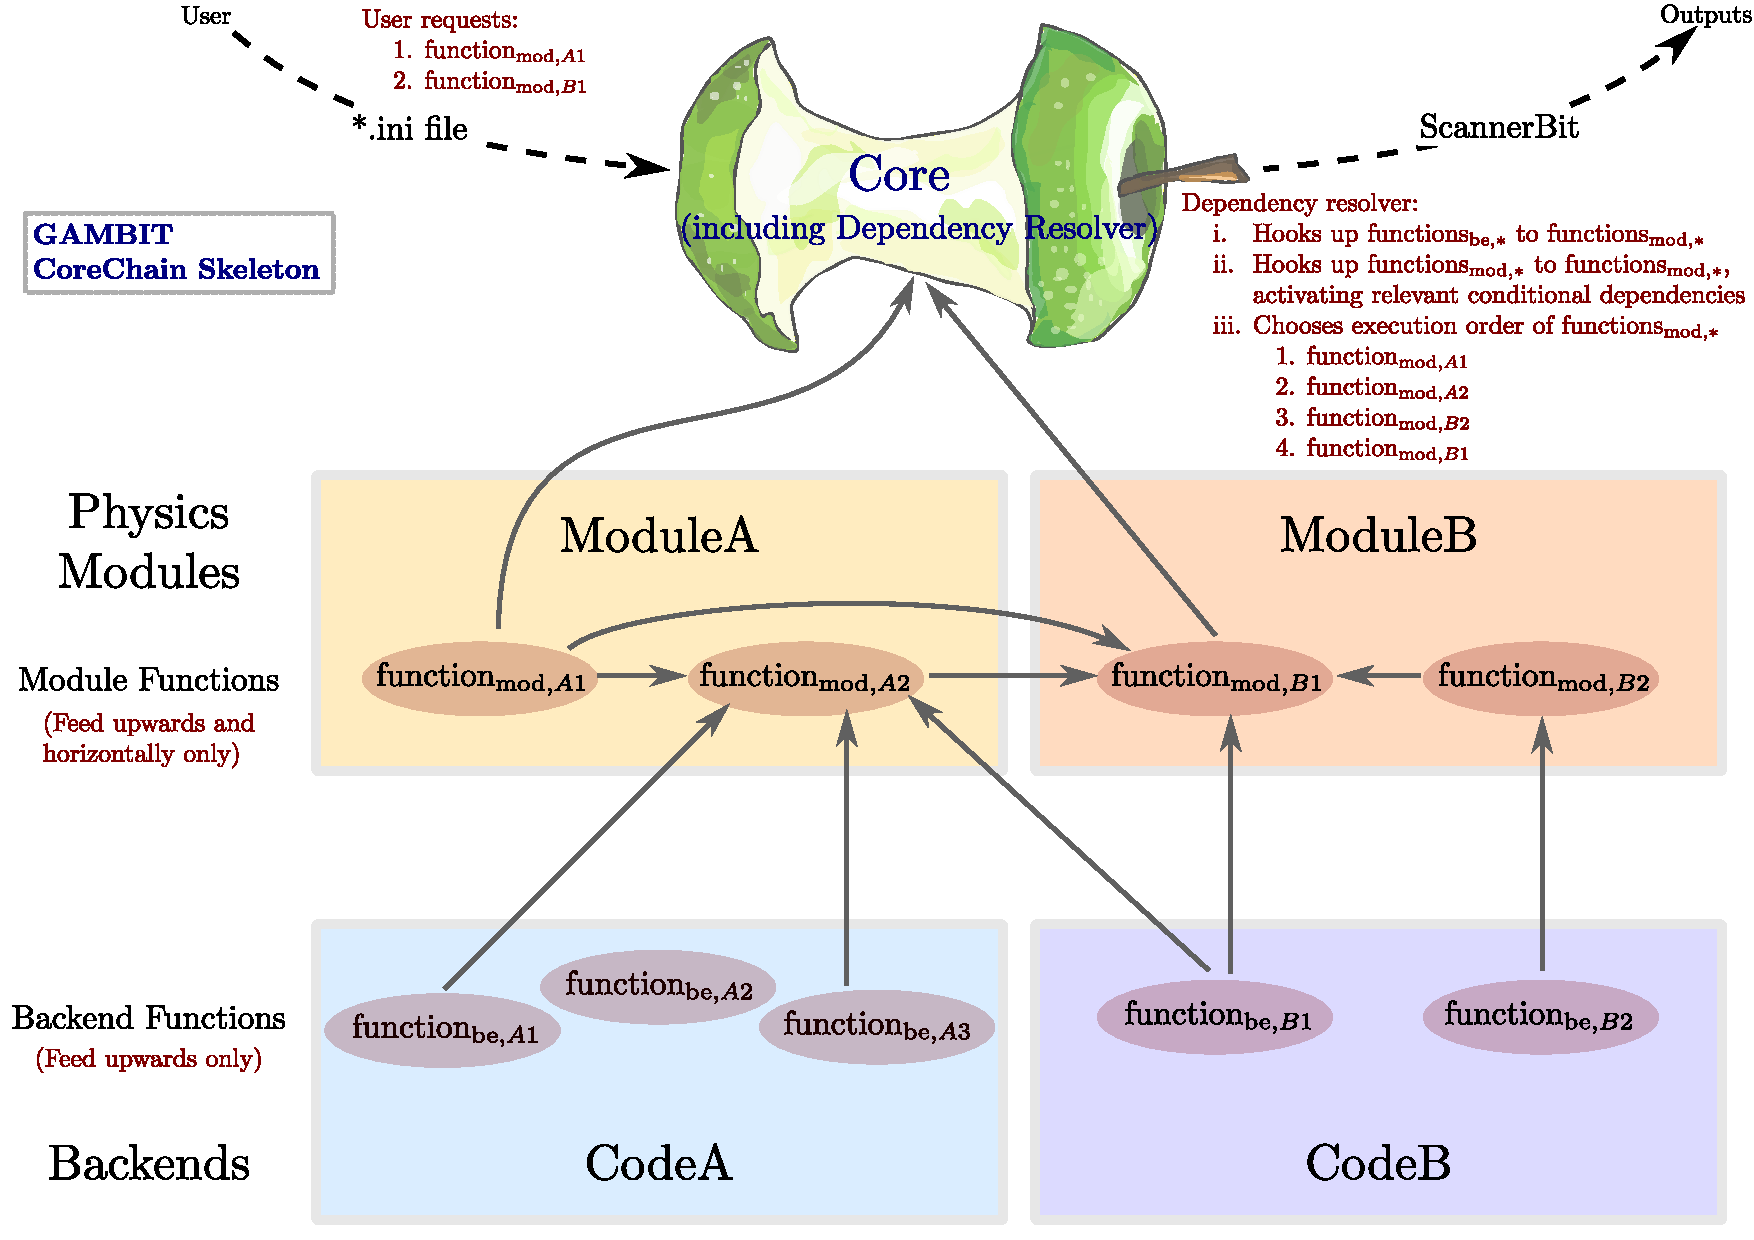
\includegraphics[width=\linewidth]{coreChainDiagram_basic}
\end{frame}


\begin{frame}
\frametitle{Rollcall + backends + dependency resolution \\Better example, take 2}
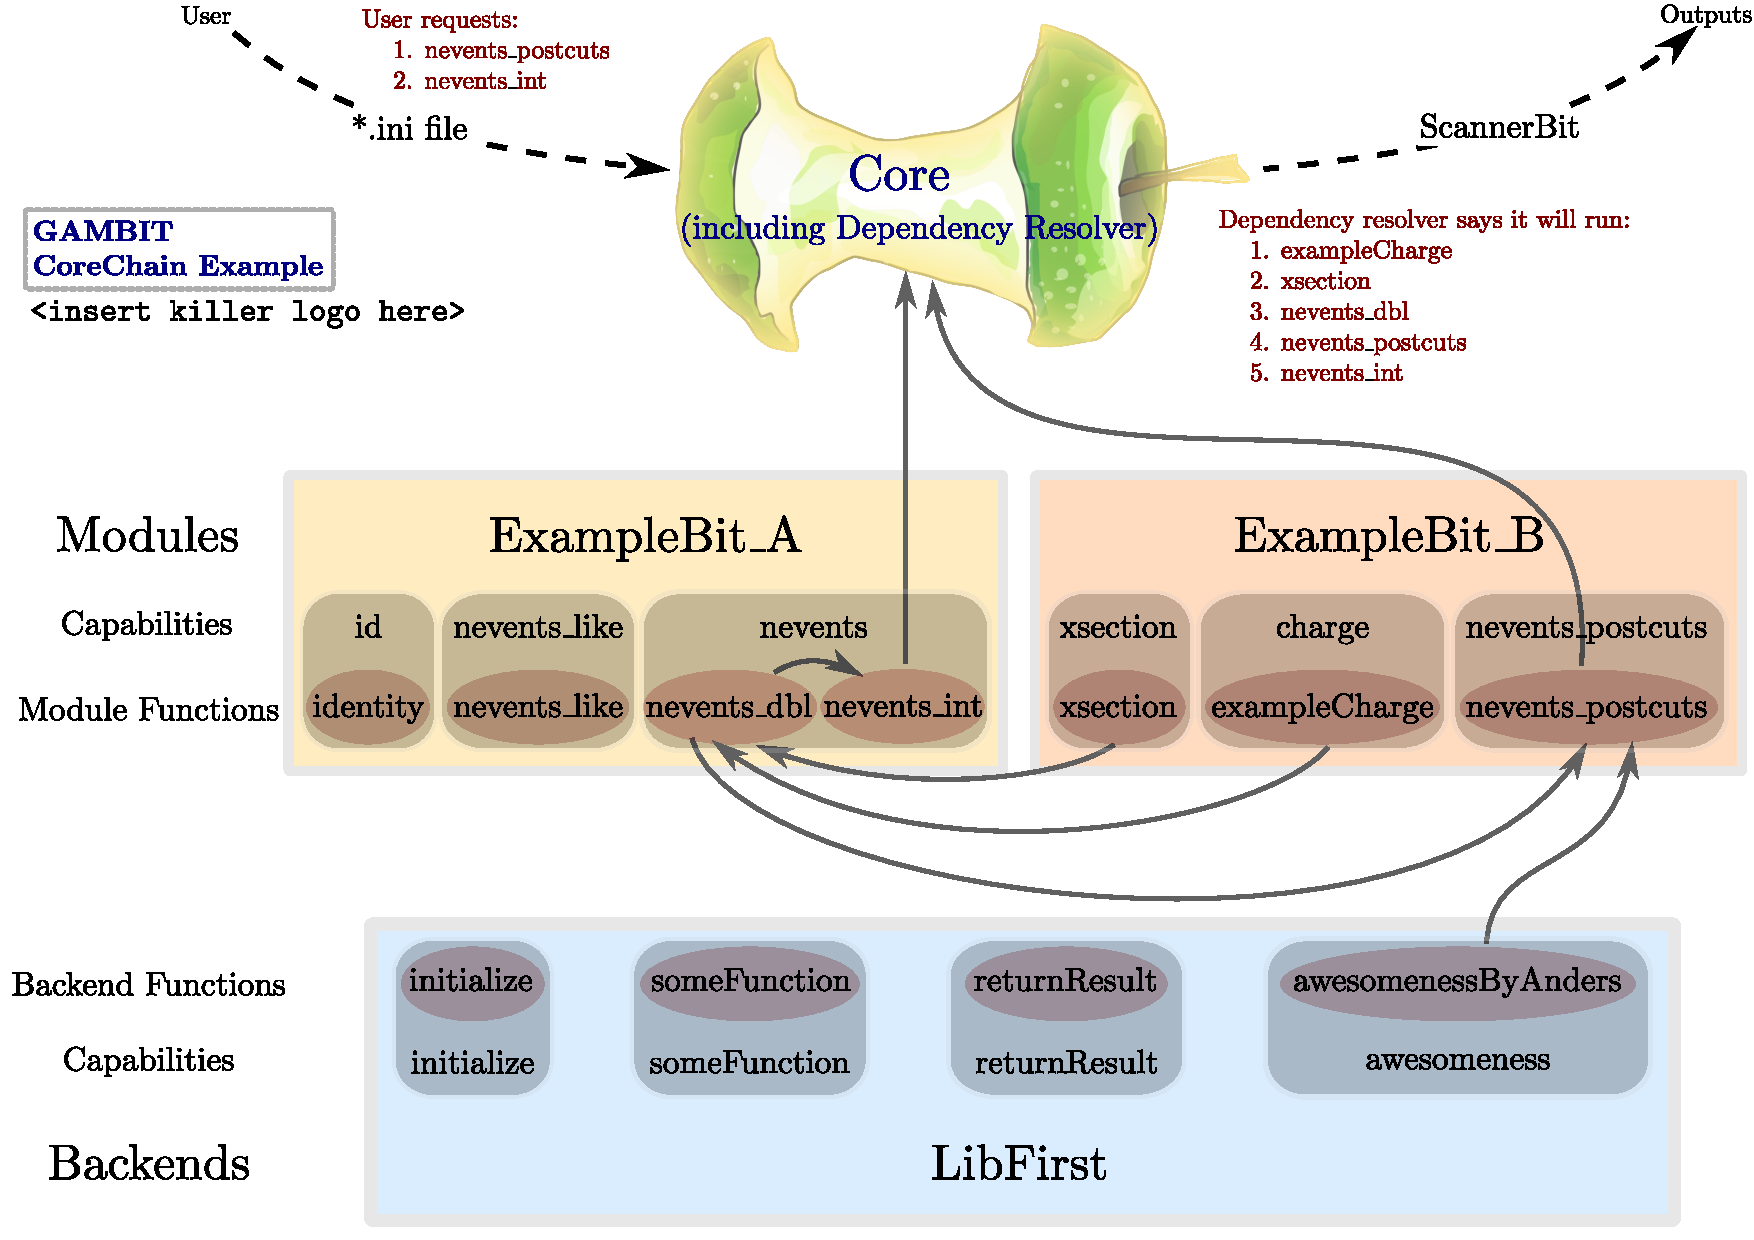
\includegraphics[width=\linewidth]{coreChainDiagram_example}
\end{frame}


\begin{frame}
\frametitle{Basic files to look at}

\small
\begin{itemize}
\item \href{run:/home/pat/gambit-hepforge/modules/Core/include/module_rollcall.hpp}{\textcolor{darkMahogany}{\texttt{modules/Core/include/module\_rollcall.hpp}}}
\item \href{run:/home/pat/gambit-hepforge/modules/Core/include/backend_rollcall.hpp}{\textcolor{darkMahogany}{\texttt{modules/Core/include/backend\_rollcall.hpp}}}
\item \href{run:/home/pat/gambit-hepforge/modules/ExampleBit_A/include/ExampleBit_A.hpp}{\textcolor{darkMahogany}{\texttt{modules/ExampleBit\_A/include/ExampleBit\_A.hpp}}}
\item \href{run:/home/pat/gambit-hepforge/modules/ExampleBit_A/src/ExampleBit_B.hpp}{\textcolor{darkMahogany}{\texttt{modules/ExampleBit\_A/src/ExampleBit\_B.hpp}}}
\item \href{run:/home/pat/gambit-hepforge/modules/ExampleBit_B/include/ExampleBit_A.hpp}{\textcolor{darkMahogany}{\texttt{modules/ExampleBit\_B/include/ExampleBit\_A.hpp}}}
\item \href{run:/home/pat/gambit-hepforge/modules/ExampleBit_B/src/ExampleBit_B.hpp}{\textcolor{darkMahogany}{\texttt{modules/ExampleBit\_B/src/ExampleBit\_B.hpp}}}
\item \href{run:/home/pat/gambit-hepforge/modules/Backends/include/backend_libfirst.hpp}{\textcolor{darkMahogany}{\texttt{modules/Backends/include/backend\_libfirst.hpp}}}
\item \href{run:/home/pat/gambit-hepforge/modules/Backends/lib/libfirst.cpp}{\textcolor{darkMahogany}{\texttt{modules/Backends/lib/libfirst.cpp}}}
\end{itemize}



\end{frame}


\end{document}

